% Created by tikzDevice version 0.12.3 on 2020-01-31 10:34:03
% !TEX encoding = UTF-8 Unicode
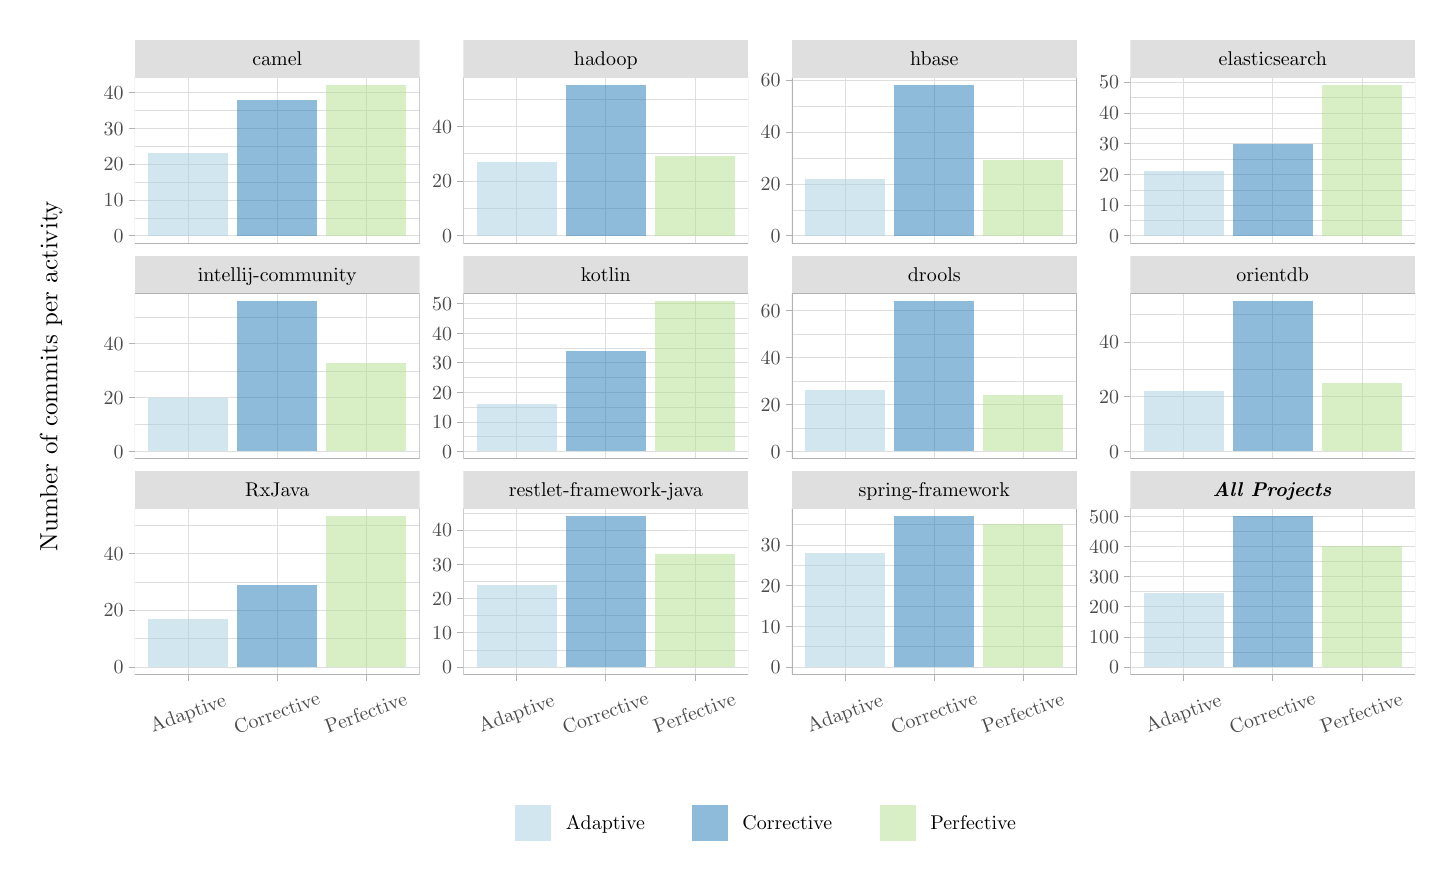
\begin{tikzpicture}[x=1pt,y=1pt]
\definecolor{fillColor}{RGB}{255,255,255}
\path[use as bounding box,fill=fillColor,fill opacity=0.00] (0,0) rectangle (505.89,303.53);
\begin{scope}
\path[clip] (  0.00,  0.00) rectangle (505.89,303.53);
\definecolor{drawColor}{RGB}{255,255,255}
\definecolor{fillColor}{RGB}{255,255,255}

\path[draw=drawColor,line width= 0.5pt,line join=round,line cap=round,fill=fillColor] (  0.00,  0.00) rectangle (505.89,303.53);
\end{scope}
\begin{scope}
\path[clip] ( 38.70,225.63) rectangle (141.66,285.48);
\definecolor{fillColor}{RGB}{255,255,255}

\path[fill=fillColor] ( 38.70,225.63) rectangle (141.66,285.48);
\definecolor{drawColor}{gray}{0.87}

\path[draw=drawColor,line width= 0.1pt,line join=round] ( 38.70,234.83) --
	(141.66,234.83);

\path[draw=drawColor,line width= 0.1pt,line join=round] ( 38.70,247.78) --
	(141.66,247.78);

\path[draw=drawColor,line width= 0.1pt,line join=round] ( 38.70,260.73) --
	(141.66,260.73);

\path[draw=drawColor,line width= 0.1pt,line join=round] ( 38.70,273.69) --
	(141.66,273.69);

\path[draw=drawColor,line width= 0.2pt,line join=round] ( 38.70,228.35) --
	(141.66,228.35);

\path[draw=drawColor,line width= 0.2pt,line join=round] ( 38.70,241.30) --
	(141.66,241.30);

\path[draw=drawColor,line width= 0.2pt,line join=round] ( 38.70,254.26) --
	(141.66,254.26);

\path[draw=drawColor,line width= 0.2pt,line join=round] ( 38.70,267.21) --
	(141.66,267.21);

\path[draw=drawColor,line width= 0.2pt,line join=round] ( 38.70,280.16) --
	(141.66,280.16);

\path[draw=drawColor,line width= 0.2pt,line join=round] ( 58.00,225.63) --
	( 58.00,285.48);

\path[draw=drawColor,line width= 0.2pt,line join=round] ( 90.18,225.63) --
	( 90.18,285.48);

\path[draw=drawColor,line width= 0.2pt,line join=round] (122.35,225.63) --
	(122.35,285.48);
\definecolor{fillColor}{RGB}{166,206,227}

\path[fill=fillColor,fill opacity=0.50] ( 43.52,228.35) rectangle ( 72.48,258.14);
\definecolor{fillColor}{RGB}{31,120,180}

\path[fill=fillColor,fill opacity=0.50] ( 75.70,228.35) rectangle (104.66,277.57);
\definecolor{fillColor}{RGB}{178,223,138}

\path[fill=fillColor,fill opacity=0.50] (107.87,228.35) rectangle (136.83,282.76);
\definecolor{drawColor}{gray}{0.70}

\path[draw=drawColor,line width= 0.5pt,line join=round,line cap=round] ( 38.70,225.63) rectangle (141.66,285.48);
\end{scope}
\begin{scope}
\path[clip] ( 38.70,147.73) rectangle (141.66,207.57);
\definecolor{fillColor}{RGB}{255,255,255}

\path[fill=fillColor] ( 38.70,147.73) rectangle (141.66,207.57);
\definecolor{drawColor}{gray}{0.87}

\path[draw=drawColor,line width= 0.1pt,line join=round] ( 38.70,160.16) --
	(141.66,160.16);

\path[draw=drawColor,line width= 0.1pt,line join=round] ( 38.70,179.59) --
	(141.66,179.59);

\path[draw=drawColor,line width= 0.1pt,line join=round] ( 38.70,199.02) --
	(141.66,199.02);

\path[draw=drawColor,line width= 0.2pt,line join=round] ( 38.70,150.45) --
	(141.66,150.45);

\path[draw=drawColor,line width= 0.2pt,line join=round] ( 38.70,169.88) --
	(141.66,169.88);

\path[draw=drawColor,line width= 0.2pt,line join=round] ( 38.70,189.31) --
	(141.66,189.31);

\path[draw=drawColor,line width= 0.2pt,line join=round] ( 58.00,147.73) --
	( 58.00,207.57);

\path[draw=drawColor,line width= 0.2pt,line join=round] ( 90.18,147.73) --
	( 90.18,207.57);

\path[draw=drawColor,line width= 0.2pt,line join=round] (122.35,147.73) --
	(122.35,207.57);
\definecolor{fillColor}{RGB}{166,206,227}

\path[fill=fillColor,fill opacity=0.50] ( 43.52,150.45) rectangle ( 72.48,169.88);
\definecolor{fillColor}{RGB}{31,120,180}

\path[fill=fillColor,fill opacity=0.50] ( 75.70,150.45) rectangle (104.66,204.85);
\definecolor{fillColor}{RGB}{178,223,138}

\path[fill=fillColor,fill opacity=0.50] (107.87,150.45) rectangle (136.83,182.51);
\definecolor{drawColor}{gray}{0.70}

\path[draw=drawColor,line width= 0.5pt,line join=round,line cap=round] ( 38.70,147.73) rectangle (141.66,207.57);
\end{scope}
\begin{scope}
\path[clip] ( 38.70, 69.82) rectangle (141.66,129.67);
\definecolor{fillColor}{RGB}{255,255,255}

\path[fill=fillColor] ( 38.70, 69.82) rectangle (141.66,129.67);
\definecolor{drawColor}{gray}{0.87}

\path[draw=drawColor,line width= 0.1pt,line join=round] ( 38.70, 82.81) --
	(141.66, 82.81);

\path[draw=drawColor,line width= 0.1pt,line join=round] ( 38.70,103.34) --
	(141.66,103.34);

\path[draw=drawColor,line width= 0.1pt,line join=round] ( 38.70,123.87) --
	(141.66,123.87);

\path[draw=drawColor,line width= 0.2pt,line join=round] ( 38.70, 72.54) --
	(141.66, 72.54);

\path[draw=drawColor,line width= 0.2pt,line join=round] ( 38.70, 93.07) --
	(141.66, 93.07);

\path[draw=drawColor,line width= 0.2pt,line join=round] ( 38.70,113.60) --
	(141.66,113.60);

\path[draw=drawColor,line width= 0.2pt,line join=round] ( 58.00, 69.82) --
	( 58.00,129.67);

\path[draw=drawColor,line width= 0.2pt,line join=round] ( 90.18, 69.82) --
	( 90.18,129.67);

\path[draw=drawColor,line width= 0.2pt,line join=round] (122.35, 69.82) --
	(122.35,129.67);
\definecolor{fillColor}{RGB}{166,206,227}

\path[fill=fillColor,fill opacity=0.50] ( 43.52, 72.54) rectangle ( 72.48, 89.99);
\definecolor{fillColor}{RGB}{31,120,180}

\path[fill=fillColor,fill opacity=0.50] ( 75.70, 72.54) rectangle (104.66,102.31);
\definecolor{fillColor}{RGB}{178,223,138}

\path[fill=fillColor,fill opacity=0.50] (107.87, 72.54) rectangle (136.83,126.95);
\definecolor{drawColor}{gray}{0.70}

\path[draw=drawColor,line width= 0.5pt,line join=round,line cap=round] ( 38.70, 69.82) rectangle (141.66,129.67);
\end{scope}
\begin{scope}
\path[clip] (157.41,225.63) rectangle (260.37,285.48);
\definecolor{fillColor}{RGB}{255,255,255}

\path[fill=fillColor] (157.41,225.63) rectangle (260.37,285.48);
\definecolor{drawColor}{gray}{0.87}

\path[draw=drawColor,line width= 0.1pt,line join=round] (157.41,238.24) --
	(260.37,238.24);

\path[draw=drawColor,line width= 0.1pt,line join=round] (157.41,258.03) --
	(260.37,258.03);

\path[draw=drawColor,line width= 0.1pt,line join=round] (157.41,277.81) --
	(260.37,277.81);

\path[draw=drawColor,line width= 0.2pt,line join=round] (157.41,228.35) --
	(260.37,228.35);

\path[draw=drawColor,line width= 0.2pt,line join=round] (157.41,248.13) --
	(260.37,248.13);

\path[draw=drawColor,line width= 0.2pt,line join=round] (157.41,267.92) --
	(260.37,267.92);

\path[draw=drawColor,line width= 0.2pt,line join=round] (176.71,225.63) --
	(176.71,285.48);

\path[draw=drawColor,line width= 0.2pt,line join=round] (208.89,225.63) --
	(208.89,285.48);

\path[draw=drawColor,line width= 0.2pt,line join=round] (241.06,225.63) --
	(241.06,285.48);
\definecolor{fillColor}{RGB}{166,206,227}

\path[fill=fillColor,fill opacity=0.50] (162.23,228.35) rectangle (191.19,255.06);
\definecolor{fillColor}{RGB}{31,120,180}

\path[fill=fillColor,fill opacity=0.50] (194.41,228.35) rectangle (223.37,282.76);
\definecolor{fillColor}{RGB}{178,223,138}

\path[fill=fillColor,fill opacity=0.50] (226.58,228.35) rectangle (255.54,257.04);
\definecolor{drawColor}{gray}{0.70}

\path[draw=drawColor,line width= 0.5pt,line join=round,line cap=round] (157.41,225.63) rectangle (260.37,285.48);
\end{scope}
\begin{scope}
\path[clip] (157.41,147.73) rectangle (260.37,207.57);
\definecolor{fillColor}{RGB}{255,255,255}

\path[fill=fillColor] (157.41,147.73) rectangle (260.37,207.57);
\definecolor{drawColor}{gray}{0.87}

\path[draw=drawColor,line width= 0.1pt,line join=round] (157.41,155.78) --
	(260.37,155.78);

\path[draw=drawColor,line width= 0.1pt,line join=round] (157.41,166.45) --
	(260.37,166.45);

\path[draw=drawColor,line width= 0.1pt,line join=round] (157.41,177.11) --
	(260.37,177.11);

\path[draw=drawColor,line width= 0.1pt,line join=round] (157.41,187.78) --
	(260.37,187.78);

\path[draw=drawColor,line width= 0.1pt,line join=round] (157.41,198.45) --
	(260.37,198.45);

\path[draw=drawColor,line width= 0.2pt,line join=round] (157.41,150.45) --
	(260.37,150.45);

\path[draw=drawColor,line width= 0.2pt,line join=round] (157.41,161.11) --
	(260.37,161.11);

\path[draw=drawColor,line width= 0.2pt,line join=round] (157.41,171.78) --
	(260.37,171.78);

\path[draw=drawColor,line width= 0.2pt,line join=round] (157.41,182.45) --
	(260.37,182.45);

\path[draw=drawColor,line width= 0.2pt,line join=round] (157.41,193.12) --
	(260.37,193.12);

\path[draw=drawColor,line width= 0.2pt,line join=round] (157.41,203.78) --
	(260.37,203.78);

\path[draw=drawColor,line width= 0.2pt,line join=round] (176.71,147.73) --
	(176.71,207.57);

\path[draw=drawColor,line width= 0.2pt,line join=round] (208.89,147.73) --
	(208.89,207.57);

\path[draw=drawColor,line width= 0.2pt,line join=round] (241.06,147.73) --
	(241.06,207.57);
\definecolor{fillColor}{RGB}{166,206,227}

\path[fill=fillColor,fill opacity=0.50] (162.23,150.45) rectangle (191.19,167.51);
\definecolor{fillColor}{RGB}{31,120,180}

\path[fill=fillColor,fill opacity=0.50] (194.41,150.45) rectangle (223.37,186.72);
\definecolor{fillColor}{RGB}{178,223,138}

\path[fill=fillColor,fill opacity=0.50] (226.58,150.45) rectangle (255.54,204.85);
\definecolor{drawColor}{gray}{0.70}

\path[draw=drawColor,line width= 0.5pt,line join=round,line cap=round] (157.41,147.73) rectangle (260.37,207.57);
\end{scope}
\begin{scope}
\path[clip] (157.41, 69.82) rectangle (260.37,129.67);
\definecolor{fillColor}{RGB}{255,255,255}

\path[fill=fillColor] (157.41, 69.82) rectangle (260.37,129.67);
\definecolor{drawColor}{gray}{0.87}

\path[draw=drawColor,line width= 0.1pt,line join=round] (157.41, 78.72) --
	(260.37, 78.72);

\path[draw=drawColor,line width= 0.1pt,line join=round] (157.41, 91.09) --
	(260.37, 91.09);

\path[draw=drawColor,line width= 0.1pt,line join=round] (157.41,103.45) --
	(260.37,103.45);

\path[draw=drawColor,line width= 0.1pt,line join=round] (157.41,115.82) --
	(260.37,115.82);

\path[draw=drawColor,line width= 0.1pt,line join=round] (157.41,128.18) --
	(260.37,128.18);

\path[draw=drawColor,line width= 0.2pt,line join=round] (157.41, 72.54) --
	(260.37, 72.54);

\path[draw=drawColor,line width= 0.2pt,line join=round] (157.41, 84.91) --
	(260.37, 84.91);

\path[draw=drawColor,line width= 0.2pt,line join=round] (157.41, 97.27) --
	(260.37, 97.27);

\path[draw=drawColor,line width= 0.2pt,line join=round] (157.41,109.64) --
	(260.37,109.64);

\path[draw=drawColor,line width= 0.2pt,line join=round] (157.41,122.00) --
	(260.37,122.00);

\path[draw=drawColor,line width= 0.2pt,line join=round] (176.71, 69.82) --
	(176.71,129.67);

\path[draw=drawColor,line width= 0.2pt,line join=round] (208.89, 69.82) --
	(208.89,129.67);

\path[draw=drawColor,line width= 0.2pt,line join=round] (241.06, 69.82) --
	(241.06,129.67);
\definecolor{fillColor}{RGB}{166,206,227}

\path[fill=fillColor,fill opacity=0.50] (162.23, 72.54) rectangle (191.19,102.22);
\definecolor{fillColor}{RGB}{31,120,180}

\path[fill=fillColor,fill opacity=0.50] (194.41, 72.54) rectangle (223.37,126.95);
\definecolor{fillColor}{RGB}{178,223,138}

\path[fill=fillColor,fill opacity=0.50] (226.58, 72.54) rectangle (255.54,113.35);
\definecolor{drawColor}{gray}{0.70}

\path[draw=drawColor,line width= 0.5pt,line join=round,line cap=round] (157.41, 69.82) rectangle (260.37,129.67);
\end{scope}
\begin{scope}
\path[clip] (276.12,225.63) rectangle (379.08,285.48);
\definecolor{fillColor}{RGB}{255,255,255}

\path[fill=fillColor] (276.12,225.63) rectangle (379.08,285.48);
\definecolor{drawColor}{gray}{0.87}

\path[draw=drawColor,line width= 0.1pt,line join=round] (276.12,237.73) --
	(379.08,237.73);

\path[draw=drawColor,line width= 0.1pt,line join=round] (276.12,256.49) --
	(379.08,256.49);

\path[draw=drawColor,line width= 0.1pt,line join=round] (276.12,275.25) --
	(379.08,275.25);

\path[draw=drawColor,line width= 0.2pt,line join=round] (276.12,228.35) --
	(379.08,228.35);

\path[draw=drawColor,line width= 0.2pt,line join=round] (276.12,247.11) --
	(379.08,247.11);

\path[draw=drawColor,line width= 0.2pt,line join=round] (276.12,265.87) --
	(379.08,265.87);

\path[draw=drawColor,line width= 0.2pt,line join=round] (276.12,284.63) --
	(379.08,284.63);

\path[draw=drawColor,line width= 0.2pt,line join=round] (295.42,225.63) --
	(295.42,285.48);

\path[draw=drawColor,line width= 0.2pt,line join=round] (327.60,225.63) --
	(327.60,285.48);

\path[draw=drawColor,line width= 0.2pt,line join=round] (359.77,225.63) --
	(359.77,285.48);
\definecolor{fillColor}{RGB}{166,206,227}

\path[fill=fillColor,fill opacity=0.50] (280.94,228.35) rectangle (309.90,248.99);
\definecolor{fillColor}{RGB}{31,120,180}

\path[fill=fillColor,fill opacity=0.50] (313.12,228.35) rectangle (342.08,282.76);
\definecolor{fillColor}{RGB}{178,223,138}

\path[fill=fillColor,fill opacity=0.50] (345.30,228.35) rectangle (374.25,255.55);
\definecolor{drawColor}{gray}{0.70}

\path[draw=drawColor,line width= 0.5pt,line join=round,line cap=round] (276.12,225.63) rectangle (379.08,285.48);
\end{scope}
\begin{scope}
\path[clip] (276.12,147.73) rectangle (379.08,207.57);
\definecolor{fillColor}{RGB}{255,255,255}

\path[fill=fillColor] (276.12,147.73) rectangle (379.08,207.57);
\definecolor{drawColor}{gray}{0.87}

\path[draw=drawColor,line width= 0.1pt,line join=round] (276.12,158.95) --
	(379.08,158.95);

\path[draw=drawColor,line width= 0.1pt,line join=round] (276.12,175.95) --
	(379.08,175.95);

\path[draw=drawColor,line width= 0.1pt,line join=round] (276.12,192.95) --
	(379.08,192.95);

\path[draw=drawColor,line width= 0.2pt,line join=round] (276.12,150.45) --
	(379.08,150.45);

\path[draw=drawColor,line width= 0.2pt,line join=round] (276.12,167.45) --
	(379.08,167.45);

\path[draw=drawColor,line width= 0.2pt,line join=round] (276.12,184.45) --
	(379.08,184.45);

\path[draw=drawColor,line width= 0.2pt,line join=round] (276.12,201.45) --
	(379.08,201.45);

\path[draw=drawColor,line width= 0.2pt,line join=round] (295.42,147.73) --
	(295.42,207.57);

\path[draw=drawColor,line width= 0.2pt,line join=round] (327.60,147.73) --
	(327.60,207.57);

\path[draw=drawColor,line width= 0.2pt,line join=round] (359.77,147.73) --
	(359.77,207.57);
\definecolor{fillColor}{RGB}{166,206,227}

\path[fill=fillColor,fill opacity=0.50] (280.94,150.45) rectangle (309.90,172.55);
\definecolor{fillColor}{RGB}{31,120,180}

\path[fill=fillColor,fill opacity=0.50] (313.12,150.45) rectangle (342.08,204.85);
\definecolor{fillColor}{RGB}{178,223,138}

\path[fill=fillColor,fill opacity=0.50] (345.30,150.45) rectangle (374.25,170.85);
\definecolor{drawColor}{gray}{0.70}

\path[draw=drawColor,line width= 0.5pt,line join=round,line cap=round] (276.12,147.73) rectangle (379.08,207.57);
\end{scope}
\begin{scope}
\path[clip] (276.12, 69.82) rectangle (379.08,129.67);
\definecolor{fillColor}{RGB}{255,255,255}

\path[fill=fillColor] (276.12, 69.82) rectangle (379.08,129.67);
\definecolor{drawColor}{gray}{0.87}

\path[draw=drawColor,line width= 0.1pt,line join=round] (276.12, 79.89) --
	(379.08, 79.89);

\path[draw=drawColor,line width= 0.1pt,line join=round] (276.12, 94.60) --
	(379.08, 94.60);

\path[draw=drawColor,line width= 0.1pt,line join=round] (276.12,109.30) --
	(379.08,109.30);

\path[draw=drawColor,line width= 0.1pt,line join=round] (276.12,124.01) --
	(379.08,124.01);

\path[draw=drawColor,line width= 0.2pt,line join=round] (276.12, 72.54) --
	(379.08, 72.54);

\path[draw=drawColor,line width= 0.2pt,line join=round] (276.12, 87.25) --
	(379.08, 87.25);

\path[draw=drawColor,line width= 0.2pt,line join=round] (276.12,101.95) --
	(379.08,101.95);

\path[draw=drawColor,line width= 0.2pt,line join=round] (276.12,116.65) --
	(379.08,116.65);

\path[draw=drawColor,line width= 0.2pt,line join=round] (295.42, 69.82) --
	(295.42,129.67);

\path[draw=drawColor,line width= 0.2pt,line join=round] (327.60, 69.82) --
	(327.60,129.67);

\path[draw=drawColor,line width= 0.2pt,line join=round] (359.77, 69.82) --
	(359.77,129.67);
\definecolor{fillColor}{RGB}{166,206,227}

\path[fill=fillColor,fill opacity=0.50] (280.94, 72.54) rectangle (309.90,113.71);
\definecolor{fillColor}{RGB}{31,120,180}

\path[fill=fillColor,fill opacity=0.50] (313.12, 72.54) rectangle (342.08,126.95);
\definecolor{fillColor}{RGB}{178,223,138}

\path[fill=fillColor,fill opacity=0.50] (345.30, 72.54) rectangle (374.25,124.01);
\definecolor{drawColor}{gray}{0.70}

\path[draw=drawColor,line width= 0.5pt,line join=round,line cap=round] (276.12, 69.82) rectangle (379.08,129.67);
\end{scope}
\begin{scope}
\path[clip] (398.43,225.63) rectangle (501.39,285.48);
\definecolor{fillColor}{RGB}{255,255,255}

\path[fill=fillColor] (398.43,225.63) rectangle (501.39,285.48);
\definecolor{drawColor}{gray}{0.87}

\path[draw=drawColor,line width= 0.1pt,line join=round] (398.43,233.90) --
	(501.39,233.90);

\path[draw=drawColor,line width= 0.1pt,line join=round] (398.43,245.00) --
	(501.39,245.00);

\path[draw=drawColor,line width= 0.1pt,line join=round] (398.43,256.11) --
	(501.39,256.11);

\path[draw=drawColor,line width= 0.1pt,line join=round] (398.43,267.21) --
	(501.39,267.21);

\path[draw=drawColor,line width= 0.1pt,line join=round] (398.43,278.31) --
	(501.39,278.31);

\path[draw=drawColor,line width= 0.2pt,line join=round] (398.43,228.35) --
	(501.39,228.35);

\path[draw=drawColor,line width= 0.2pt,line join=round] (398.43,239.45) --
	(501.39,239.45);

\path[draw=drawColor,line width= 0.2pt,line join=round] (398.43,250.56) --
	(501.39,250.56);

\path[draw=drawColor,line width= 0.2pt,line join=round] (398.43,261.66) --
	(501.39,261.66);

\path[draw=drawColor,line width= 0.2pt,line join=round] (398.43,272.76) --
	(501.39,272.76);

\path[draw=drawColor,line width= 0.2pt,line join=round] (398.43,283.87) --
	(501.39,283.87);

\path[draw=drawColor,line width= 0.2pt,line join=round] (417.73,225.63) --
	(417.73,285.48);

\path[draw=drawColor,line width= 0.2pt,line join=round] (449.91,225.63) --
	(449.91,285.48);

\path[draw=drawColor,line width= 0.2pt,line join=round] (482.08,225.63) --
	(482.08,285.48);
\definecolor{fillColor}{RGB}{166,206,227}

\path[fill=fillColor,fill opacity=0.50] (403.25,228.35) rectangle (432.21,251.67);
\definecolor{fillColor}{RGB}{31,120,180}

\path[fill=fillColor,fill opacity=0.50] (435.43,228.35) rectangle (464.39,261.66);
\definecolor{fillColor}{RGB}{178,223,138}

\path[fill=fillColor,fill opacity=0.50] (467.61,228.35) rectangle (496.56,282.76);
\definecolor{drawColor}{gray}{0.70}

\path[draw=drawColor,line width= 0.5pt,line join=round,line cap=round] (398.43,225.63) rectangle (501.39,285.48);
\end{scope}
\begin{scope}
\path[clip] (398.43,147.73) rectangle (501.39,207.57);
\definecolor{fillColor}{RGB}{255,255,255}

\path[fill=fillColor] (398.43,147.73) rectangle (501.39,207.57);
\definecolor{drawColor}{gray}{0.87}

\path[draw=drawColor,line width= 0.1pt,line join=round] (398.43,160.34) --
	(501.39,160.34);

\path[draw=drawColor,line width= 0.1pt,line join=round] (398.43,180.12) --
	(501.39,180.12);

\path[draw=drawColor,line width= 0.1pt,line join=round] (398.43,199.91) --
	(501.39,199.91);

\path[draw=drawColor,line width= 0.2pt,line join=round] (398.43,150.45) --
	(501.39,150.45);

\path[draw=drawColor,line width= 0.2pt,line join=round] (398.43,170.23) --
	(501.39,170.23);

\path[draw=drawColor,line width= 0.2pt,line join=round] (398.43,190.01) --
	(501.39,190.01);

\path[draw=drawColor,line width= 0.2pt,line join=round] (417.73,147.73) --
	(417.73,207.57);

\path[draw=drawColor,line width= 0.2pt,line join=round] (449.91,147.73) --
	(449.91,207.57);

\path[draw=drawColor,line width= 0.2pt,line join=round] (482.08,147.73) --
	(482.08,207.57);
\definecolor{fillColor}{RGB}{166,206,227}

\path[fill=fillColor,fill opacity=0.50] (403.25,150.45) rectangle (432.21,172.21);
\definecolor{fillColor}{RGB}{31,120,180}

\path[fill=fillColor,fill opacity=0.50] (435.43,150.45) rectangle (464.39,204.85);
\definecolor{fillColor}{RGB}{178,223,138}

\path[fill=fillColor,fill opacity=0.50] (467.61,150.45) rectangle (496.56,175.18);
\definecolor{drawColor}{gray}{0.70}

\path[draw=drawColor,line width= 0.5pt,line join=round,line cap=round] (398.43,147.73) rectangle (501.39,207.57);
\end{scope}
\begin{scope}
\path[clip] (398.43, 69.82) rectangle (501.39,129.67);
\definecolor{fillColor}{RGB}{255,255,255}

\path[fill=fillColor] (398.43, 69.82) rectangle (501.39,129.67);
\definecolor{drawColor}{gray}{0.87}

\path[draw=drawColor,line width= 0.1pt,line join=round] (398.43, 77.98) --
	(501.39, 77.98);

\path[draw=drawColor,line width= 0.1pt,line join=round] (398.43, 88.86) --
	(501.39, 88.86);

\path[draw=drawColor,line width= 0.1pt,line join=round] (398.43, 99.74) --
	(501.39, 99.74);

\path[draw=drawColor,line width= 0.1pt,line join=round] (398.43,110.63) --
	(501.39,110.63);

\path[draw=drawColor,line width= 0.1pt,line join=round] (398.43,121.51) --
	(501.39,121.51);

\path[draw=drawColor,line width= 0.2pt,line join=round] (398.43, 72.54) --
	(501.39, 72.54);

\path[draw=drawColor,line width= 0.2pt,line join=round] (398.43, 83.42) --
	(501.39, 83.42);

\path[draw=drawColor,line width= 0.2pt,line join=round] (398.43, 94.30) --
	(501.39, 94.30);

\path[draw=drawColor,line width= 0.2pt,line join=round] (398.43,105.18) --
	(501.39,105.18);

\path[draw=drawColor,line width= 0.2pt,line join=round] (398.43,116.07) --
	(501.39,116.07);

\path[draw=drawColor,line width= 0.2pt,line join=round] (398.43,126.95) --
	(501.39,126.95);

\path[draw=drawColor,line width= 0.2pt,line join=round] (417.73, 69.82) --
	(417.73,129.67);

\path[draw=drawColor,line width= 0.2pt,line join=round] (449.91, 69.82) --
	(449.91,129.67);

\path[draw=drawColor,line width= 0.2pt,line join=round] (482.08, 69.82) --
	(482.08,129.67);
\definecolor{fillColor}{RGB}{166,206,227}

\path[fill=fillColor,fill opacity=0.50] (403.25, 72.54) rectangle (432.21, 99.31);
\definecolor{fillColor}{RGB}{31,120,180}

\path[fill=fillColor,fill opacity=0.50] (435.43, 72.54) rectangle (464.39,126.95);
\definecolor{fillColor}{RGB}{178,223,138}

\path[fill=fillColor,fill opacity=0.50] (467.61, 72.54) rectangle (496.56,116.39);
\definecolor{drawColor}{gray}{0.70}

\path[draw=drawColor,line width= 0.5pt,line join=round,line cap=round] (398.43, 69.82) rectangle (501.39,129.67);
\end{scope}
\begin{scope}
\path[clip] ( 38.70,129.67) rectangle (141.66,143.23);
\definecolor{fillColor}{RGB}{223,223,223}

\path[fill=fillColor] ( 38.70,129.67) rectangle (141.66,143.23);
\definecolor{drawColor}{RGB}{0,0,0}

\node[text=drawColor,anchor=base,inner sep=0pt, outer sep=0pt, scale=  0.72] at ( 90.18,133.97) {RxJava};
\end{scope}
\begin{scope}
\path[clip] (157.41,129.67) rectangle (260.37,143.23);
\definecolor{fillColor}{RGB}{223,223,223}

\path[fill=fillColor] (157.41,129.67) rectangle (260.37,143.23);
\definecolor{drawColor}{RGB}{0,0,0}

\node[text=drawColor,anchor=base,inner sep=0pt, outer sep=0pt, scale=  0.72] at (208.89,133.97) {restlet-framework-java};
\end{scope}
\begin{scope}
\path[clip] (276.12,129.67) rectangle (379.08,143.23);
\definecolor{fillColor}{RGB}{223,223,223}

\path[fill=fillColor] (276.12,129.67) rectangle (379.08,143.23);
\definecolor{drawColor}{RGB}{0,0,0}

\node[text=drawColor,anchor=base,inner sep=0pt, outer sep=0pt, scale=  0.72] at (327.60,133.97) {spring-framework};
\end{scope}
\begin{scope}
\path[clip] (398.43,129.67) rectangle (501.39,143.23);
\definecolor{fillColor}{RGB}{223,223,223}

\path[fill=fillColor] (398.43,129.67) rectangle (501.39,143.23);
\definecolor{drawColor}{RGB}{0,0,0}

\node[text=drawColor,anchor=base,inner sep=0pt, outer sep=0pt, scale=  0.72] at (449.91,133.97) {\textbf{\emph{All Projects}}};
\end{scope}
\begin{scope}
\path[clip] ( 38.70,207.57) rectangle (141.66,221.13);
\definecolor{fillColor}{RGB}{223,223,223}

\path[fill=fillColor] ( 38.70,207.57) rectangle (141.66,221.13);
\definecolor{drawColor}{RGB}{0,0,0}

\node[text=drawColor,anchor=base,inner sep=0pt, outer sep=0pt, scale=  0.72] at ( 90.18,211.87) {intellij-community};
\end{scope}
\begin{scope}
\path[clip] (157.41,207.57) rectangle (260.37,221.13);
\definecolor{fillColor}{RGB}{223,223,223}

\path[fill=fillColor] (157.41,207.57) rectangle (260.37,221.13);
\definecolor{drawColor}{RGB}{0,0,0}

\node[text=drawColor,anchor=base,inner sep=0pt, outer sep=0pt, scale=  0.72] at (208.89,211.87) {kotlin};
\end{scope}
\begin{scope}
\path[clip] (276.12,207.57) rectangle (379.08,221.13);
\definecolor{fillColor}{RGB}{223,223,223}

\path[fill=fillColor] (276.12,207.57) rectangle (379.08,221.13);
\definecolor{drawColor}{RGB}{0,0,0}

\node[text=drawColor,anchor=base,inner sep=0pt, outer sep=0pt, scale=  0.72] at (327.60,211.87) {drools};
\end{scope}
\begin{scope}
\path[clip] (398.43,207.57) rectangle (501.39,221.13);
\definecolor{fillColor}{RGB}{223,223,223}

\path[fill=fillColor] (398.43,207.57) rectangle (501.39,221.13);
\definecolor{drawColor}{RGB}{0,0,0}

\node[text=drawColor,anchor=base,inner sep=0pt, outer sep=0pt, scale=  0.72] at (449.91,211.87) {orientdb};
\end{scope}
\begin{scope}
\path[clip] ( 38.70,285.48) rectangle (141.66,299.03);
\definecolor{fillColor}{RGB}{223,223,223}

\path[fill=fillColor] ( 38.70,285.48) rectangle (141.66,299.03);
\definecolor{drawColor}{RGB}{0,0,0}

\node[text=drawColor,anchor=base,inner sep=0pt, outer sep=0pt, scale=  0.72] at ( 90.18,289.78) {camel};
\end{scope}
\begin{scope}
\path[clip] (157.41,285.48) rectangle (260.37,299.03);
\definecolor{fillColor}{RGB}{223,223,223}

\path[fill=fillColor] (157.41,285.48) rectangle (260.37,299.03);
\definecolor{drawColor}{RGB}{0,0,0}

\node[text=drawColor,anchor=base,inner sep=0pt, outer sep=0pt, scale=  0.72] at (208.89,289.78) {hadoop};
\end{scope}
\begin{scope}
\path[clip] (276.12,285.48) rectangle (379.08,299.03);
\definecolor{fillColor}{RGB}{223,223,223}

\path[fill=fillColor] (276.12,285.48) rectangle (379.08,299.03);
\definecolor{drawColor}{RGB}{0,0,0}

\node[text=drawColor,anchor=base,inner sep=0pt, outer sep=0pt, scale=  0.72] at (327.60,289.78) {hbase};
\end{scope}
\begin{scope}
\path[clip] (398.43,285.48) rectangle (501.39,299.03);
\definecolor{fillColor}{RGB}{223,223,223}

\path[fill=fillColor] (398.43,285.48) rectangle (501.39,299.03);
\definecolor{drawColor}{RGB}{0,0,0}

\node[text=drawColor,anchor=base,inner sep=0pt, outer sep=0pt, scale=  0.72] at (449.91,289.78) {elasticsearch};
\end{scope}
\begin{scope}
\path[clip] (  0.00,  0.00) rectangle (505.89,303.53);
\definecolor{drawColor}{gray}{0.70}

\path[draw=drawColor,line width= 0.2pt,line join=round] ( 58.00, 67.57) --
	( 58.00, 69.82);

\path[draw=drawColor,line width= 0.2pt,line join=round] ( 90.18, 67.57) --
	( 90.18, 69.82);

\path[draw=drawColor,line width= 0.2pt,line join=round] (122.35, 67.57) --
	(122.35, 69.82);
\end{scope}
\begin{scope}
\path[clip] (  0.00,  0.00) rectangle (505.89,303.53);
\definecolor{drawColor}{gray}{0.30}

\node[text=drawColor,rotate= 20.00,anchor=base,inner sep=0pt, outer sep=0pt, scale=  0.72] at ( 58.68, 53.67) {Adaptive};

\node[text=drawColor,rotate= 20.00,anchor=base,inner sep=0pt, outer sep=0pt, scale=  0.72] at ( 90.86, 53.67) {Corrective};

\node[text=drawColor,rotate= 20.00,anchor=base,inner sep=0pt, outer sep=0pt, scale=  0.72] at (123.03, 53.67) {Perfective};
\end{scope}
\begin{scope}
\path[clip] (  0.00,  0.00) rectangle (505.89,303.53);
\definecolor{drawColor}{gray}{0.70}

\path[draw=drawColor,line width= 0.2pt,line join=round] (176.71, 67.57) --
	(176.71, 69.82);

\path[draw=drawColor,line width= 0.2pt,line join=round] (208.89, 67.57) --
	(208.89, 69.82);

\path[draw=drawColor,line width= 0.2pt,line join=round] (241.06, 67.57) --
	(241.06, 69.82);
\end{scope}
\begin{scope}
\path[clip] (  0.00,  0.00) rectangle (505.89,303.53);
\definecolor{drawColor}{gray}{0.30}

\node[text=drawColor,rotate= 20.00,anchor=base,inner sep=0pt, outer sep=0pt, scale=  0.72] at (177.39, 53.67) {Adaptive};

\node[text=drawColor,rotate= 20.00,anchor=base,inner sep=0pt, outer sep=0pt, scale=  0.72] at (209.57, 53.67) {Corrective};

\node[text=drawColor,rotate= 20.00,anchor=base,inner sep=0pt, outer sep=0pt, scale=  0.72] at (241.74, 53.67) {Perfective};
\end{scope}
\begin{scope}
\path[clip] (  0.00,  0.00) rectangle (505.89,303.53);
\definecolor{drawColor}{gray}{0.70}

\path[draw=drawColor,line width= 0.2pt,line join=round] (295.42, 67.57) --
	(295.42, 69.82);

\path[draw=drawColor,line width= 0.2pt,line join=round] (327.60, 67.57) --
	(327.60, 69.82);

\path[draw=drawColor,line width= 0.2pt,line join=round] (359.77, 67.57) --
	(359.77, 69.82);
\end{scope}
\begin{scope}
\path[clip] (  0.00,  0.00) rectangle (505.89,303.53);
\definecolor{drawColor}{gray}{0.30}

\node[text=drawColor,rotate= 20.00,anchor=base,inner sep=0pt, outer sep=0pt, scale=  0.72] at (296.10, 53.67) {Adaptive};

\node[text=drawColor,rotate= 20.00,anchor=base,inner sep=0pt, outer sep=0pt, scale=  0.72] at (328.28, 53.67) {Corrective};

\node[text=drawColor,rotate= 20.00,anchor=base,inner sep=0pt, outer sep=0pt, scale=  0.72] at (360.45, 53.67) {Perfective};
\end{scope}
\begin{scope}
\path[clip] (  0.00,  0.00) rectangle (505.89,303.53);
\definecolor{drawColor}{gray}{0.70}

\path[draw=drawColor,line width= 0.2pt,line join=round] (417.73, 67.57) --
	(417.73, 69.82);

\path[draw=drawColor,line width= 0.2pt,line join=round] (449.91, 67.57) --
	(449.91, 69.82);

\path[draw=drawColor,line width= 0.2pt,line join=round] (482.08, 67.57) --
	(482.08, 69.82);
\end{scope}
\begin{scope}
\path[clip] (  0.00,  0.00) rectangle (505.89,303.53);
\definecolor{drawColor}{gray}{0.30}

\node[text=drawColor,rotate= 20.00,anchor=base,inner sep=0pt, outer sep=0pt, scale=  0.72] at (418.41, 53.67) {Adaptive};

\node[text=drawColor,rotate= 20.00,anchor=base,inner sep=0pt, outer sep=0pt, scale=  0.72] at (450.59, 53.67) {Corrective};

\node[text=drawColor,rotate= 20.00,anchor=base,inner sep=0pt, outer sep=0pt, scale=  0.72] at (482.76, 53.67) {Perfective};
\end{scope}
\begin{scope}
\path[clip] (  0.00,  0.00) rectangle (505.89,303.53);
\definecolor{drawColor}{gray}{0.30}

\node[text=drawColor,anchor=base east,inner sep=0pt, outer sep=0pt, scale=  0.72] at (394.38,225.87) {0};

\node[text=drawColor,anchor=base east,inner sep=0pt, outer sep=0pt, scale=  0.72] at (394.38,236.97) {10};

\node[text=drawColor,anchor=base east,inner sep=0pt, outer sep=0pt, scale=  0.72] at (394.38,248.08) {20};

\node[text=drawColor,anchor=base east,inner sep=0pt, outer sep=0pt, scale=  0.72] at (394.38,259.18) {30};

\node[text=drawColor,anchor=base east,inner sep=0pt, outer sep=0pt, scale=  0.72] at (394.38,270.28) {40};

\node[text=drawColor,anchor=base east,inner sep=0pt, outer sep=0pt, scale=  0.72] at (394.38,281.39) {50};
\end{scope}
\begin{scope}
\path[clip] (  0.00,  0.00) rectangle (505.89,303.53);
\definecolor{drawColor}{gray}{0.70}

\path[draw=drawColor,line width= 0.2pt,line join=round] (396.18,228.35) --
	(398.43,228.35);

\path[draw=drawColor,line width= 0.2pt,line join=round] (396.18,239.45) --
	(398.43,239.45);

\path[draw=drawColor,line width= 0.2pt,line join=round] (396.18,250.56) --
	(398.43,250.56);

\path[draw=drawColor,line width= 0.2pt,line join=round] (396.18,261.66) --
	(398.43,261.66);

\path[draw=drawColor,line width= 0.2pt,line join=round] (396.18,272.76) --
	(398.43,272.76);

\path[draw=drawColor,line width= 0.2pt,line join=round] (396.18,283.87) --
	(398.43,283.87);
\end{scope}
\begin{scope}
\path[clip] (  0.00,  0.00) rectangle (505.89,303.53);
\definecolor{drawColor}{gray}{0.30}

\node[text=drawColor,anchor=base east,inner sep=0pt, outer sep=0pt, scale=  0.72] at (394.38,147.97) {0};

\node[text=drawColor,anchor=base east,inner sep=0pt, outer sep=0pt, scale=  0.72] at (394.38,167.75) {20};

\node[text=drawColor,anchor=base east,inner sep=0pt, outer sep=0pt, scale=  0.72] at (394.38,187.53) {40};
\end{scope}
\begin{scope}
\path[clip] (  0.00,  0.00) rectangle (505.89,303.53);
\definecolor{drawColor}{gray}{0.70}

\path[draw=drawColor,line width= 0.2pt,line join=round] (396.18,150.45) --
	(398.43,150.45);

\path[draw=drawColor,line width= 0.2pt,line join=round] (396.18,170.23) --
	(398.43,170.23);

\path[draw=drawColor,line width= 0.2pt,line join=round] (396.18,190.01) --
	(398.43,190.01);
\end{scope}
\begin{scope}
\path[clip] (  0.00,  0.00) rectangle (505.89,303.53);
\definecolor{drawColor}{gray}{0.30}

\node[text=drawColor,anchor=base east,inner sep=0pt, outer sep=0pt, scale=  0.72] at (394.38, 70.06) {0};

\node[text=drawColor,anchor=base east,inner sep=0pt, outer sep=0pt, scale=  0.72] at (394.38, 80.94) {100};

\node[text=drawColor,anchor=base east,inner sep=0pt, outer sep=0pt, scale=  0.72] at (394.38, 91.82) {200};

\node[text=drawColor,anchor=base east,inner sep=0pt, outer sep=0pt, scale=  0.72] at (394.38,102.71) {300};

\node[text=drawColor,anchor=base east,inner sep=0pt, outer sep=0pt, scale=  0.72] at (394.38,113.59) {400};

\node[text=drawColor,anchor=base east,inner sep=0pt, outer sep=0pt, scale=  0.72] at (394.38,124.47) {500};
\end{scope}
\begin{scope}
\path[clip] (  0.00,  0.00) rectangle (505.89,303.53);
\definecolor{drawColor}{gray}{0.70}

\path[draw=drawColor,line width= 0.2pt,line join=round] (396.18, 72.54) --
	(398.43, 72.54);

\path[draw=drawColor,line width= 0.2pt,line join=round] (396.18, 83.42) --
	(398.43, 83.42);

\path[draw=drawColor,line width= 0.2pt,line join=round] (396.18, 94.30) --
	(398.43, 94.30);

\path[draw=drawColor,line width= 0.2pt,line join=round] (396.18,105.18) --
	(398.43,105.18);

\path[draw=drawColor,line width= 0.2pt,line join=round] (396.18,116.07) --
	(398.43,116.07);

\path[draw=drawColor,line width= 0.2pt,line join=round] (396.18,126.95) --
	(398.43,126.95);
\end{scope}
\begin{scope}
\path[clip] (  0.00,  0.00) rectangle (505.89,303.53);
\definecolor{drawColor}{gray}{0.30}

\node[text=drawColor,anchor=base east,inner sep=0pt, outer sep=0pt, scale=  0.72] at (272.07,225.87) {0};

\node[text=drawColor,anchor=base east,inner sep=0pt, outer sep=0pt, scale=  0.72] at (272.07,244.63) {20};

\node[text=drawColor,anchor=base east,inner sep=0pt, outer sep=0pt, scale=  0.72] at (272.07,263.39) {40};

\node[text=drawColor,anchor=base east,inner sep=0pt, outer sep=0pt, scale=  0.72] at (272.07,282.15) {60};
\end{scope}
\begin{scope}
\path[clip] (  0.00,  0.00) rectangle (505.89,303.53);
\definecolor{drawColor}{gray}{0.70}

\path[draw=drawColor,line width= 0.2pt,line join=round] (273.87,228.35) --
	(276.12,228.35);

\path[draw=drawColor,line width= 0.2pt,line join=round] (273.87,247.11) --
	(276.12,247.11);

\path[draw=drawColor,line width= 0.2pt,line join=round] (273.87,265.87) --
	(276.12,265.87);

\path[draw=drawColor,line width= 0.2pt,line join=round] (273.87,284.63) --
	(276.12,284.63);
\end{scope}
\begin{scope}
\path[clip] (  0.00,  0.00) rectangle (505.89,303.53);
\definecolor{drawColor}{gray}{0.30}

\node[text=drawColor,anchor=base east,inner sep=0pt, outer sep=0pt, scale=  0.72] at (272.07,147.97) {0};

\node[text=drawColor,anchor=base east,inner sep=0pt, outer sep=0pt, scale=  0.72] at (272.07,164.97) {20};

\node[text=drawColor,anchor=base east,inner sep=0pt, outer sep=0pt, scale=  0.72] at (272.07,181.97) {40};

\node[text=drawColor,anchor=base east,inner sep=0pt, outer sep=0pt, scale=  0.72] at (272.07,198.97) {60};
\end{scope}
\begin{scope}
\path[clip] (  0.00,  0.00) rectangle (505.89,303.53);
\definecolor{drawColor}{gray}{0.70}

\path[draw=drawColor,line width= 0.2pt,line join=round] (273.87,150.45) --
	(276.12,150.45);

\path[draw=drawColor,line width= 0.2pt,line join=round] (273.87,167.45) --
	(276.12,167.45);

\path[draw=drawColor,line width= 0.2pt,line join=round] (273.87,184.45) --
	(276.12,184.45);

\path[draw=drawColor,line width= 0.2pt,line join=round] (273.87,201.45) --
	(276.12,201.45);
\end{scope}
\begin{scope}
\path[clip] (  0.00,  0.00) rectangle (505.89,303.53);
\definecolor{drawColor}{gray}{0.30}

\node[text=drawColor,anchor=base east,inner sep=0pt, outer sep=0pt, scale=  0.72] at (272.07, 70.06) {0};

\node[text=drawColor,anchor=base east,inner sep=0pt, outer sep=0pt, scale=  0.72] at (272.07, 84.77) {10};

\node[text=drawColor,anchor=base east,inner sep=0pt, outer sep=0pt, scale=  0.72] at (272.07, 99.47) {20};

\node[text=drawColor,anchor=base east,inner sep=0pt, outer sep=0pt, scale=  0.72] at (272.07,114.17) {30};
\end{scope}
\begin{scope}
\path[clip] (  0.00,  0.00) rectangle (505.89,303.53);
\definecolor{drawColor}{gray}{0.70}

\path[draw=drawColor,line width= 0.2pt,line join=round] (273.87, 72.54) --
	(276.12, 72.54);

\path[draw=drawColor,line width= 0.2pt,line join=round] (273.87, 87.25) --
	(276.12, 87.25);

\path[draw=drawColor,line width= 0.2pt,line join=round] (273.87,101.95) --
	(276.12,101.95);

\path[draw=drawColor,line width= 0.2pt,line join=round] (273.87,116.65) --
	(276.12,116.65);
\end{scope}
\begin{scope}
\path[clip] (  0.00,  0.00) rectangle (505.89,303.53);
\definecolor{drawColor}{gray}{0.30}

\node[text=drawColor,anchor=base east,inner sep=0pt, outer sep=0pt, scale=  0.72] at (153.36,225.87) {0};

\node[text=drawColor,anchor=base east,inner sep=0pt, outer sep=0pt, scale=  0.72] at (153.36,245.65) {20};

\node[text=drawColor,anchor=base east,inner sep=0pt, outer sep=0pt, scale=  0.72] at (153.36,265.44) {40};
\end{scope}
\begin{scope}
\path[clip] (  0.00,  0.00) rectangle (505.89,303.53);
\definecolor{drawColor}{gray}{0.70}

\path[draw=drawColor,line width= 0.2pt,line join=round] (155.16,228.35) --
	(157.41,228.35);

\path[draw=drawColor,line width= 0.2pt,line join=round] (155.16,248.13) --
	(157.41,248.13);

\path[draw=drawColor,line width= 0.2pt,line join=round] (155.16,267.92) --
	(157.41,267.92);
\end{scope}
\begin{scope}
\path[clip] (  0.00,  0.00) rectangle (505.89,303.53);
\definecolor{drawColor}{gray}{0.30}

\node[text=drawColor,anchor=base east,inner sep=0pt, outer sep=0pt, scale=  0.72] at (153.36,147.97) {0};

\node[text=drawColor,anchor=base east,inner sep=0pt, outer sep=0pt, scale=  0.72] at (153.36,158.63) {10};

\node[text=drawColor,anchor=base east,inner sep=0pt, outer sep=0pt, scale=  0.72] at (153.36,169.30) {20};

\node[text=drawColor,anchor=base east,inner sep=0pt, outer sep=0pt, scale=  0.72] at (153.36,179.97) {30};

\node[text=drawColor,anchor=base east,inner sep=0pt, outer sep=0pt, scale=  0.72] at (153.36,190.64) {40};

\node[text=drawColor,anchor=base east,inner sep=0pt, outer sep=0pt, scale=  0.72] at (153.36,201.30) {50};
\end{scope}
\begin{scope}
\path[clip] (  0.00,  0.00) rectangle (505.89,303.53);
\definecolor{drawColor}{gray}{0.70}

\path[draw=drawColor,line width= 0.2pt,line join=round] (155.16,150.45) --
	(157.41,150.45);

\path[draw=drawColor,line width= 0.2pt,line join=round] (155.16,161.11) --
	(157.41,161.11);

\path[draw=drawColor,line width= 0.2pt,line join=round] (155.16,171.78) --
	(157.41,171.78);

\path[draw=drawColor,line width= 0.2pt,line join=round] (155.16,182.45) --
	(157.41,182.45);

\path[draw=drawColor,line width= 0.2pt,line join=round] (155.16,193.12) --
	(157.41,193.12);

\path[draw=drawColor,line width= 0.2pt,line join=round] (155.16,203.78) --
	(157.41,203.78);
\end{scope}
\begin{scope}
\path[clip] (  0.00,  0.00) rectangle (505.89,303.53);
\definecolor{drawColor}{gray}{0.30}

\node[text=drawColor,anchor=base east,inner sep=0pt, outer sep=0pt, scale=  0.72] at (153.36, 70.06) {0};

\node[text=drawColor,anchor=base east,inner sep=0pt, outer sep=0pt, scale=  0.72] at (153.36, 82.43) {10};

\node[text=drawColor,anchor=base east,inner sep=0pt, outer sep=0pt, scale=  0.72] at (153.36, 94.79) {20};

\node[text=drawColor,anchor=base east,inner sep=0pt, outer sep=0pt, scale=  0.72] at (153.36,107.16) {30};

\node[text=drawColor,anchor=base east,inner sep=0pt, outer sep=0pt, scale=  0.72] at (153.36,119.52) {40};
\end{scope}
\begin{scope}
\path[clip] (  0.00,  0.00) rectangle (505.89,303.53);
\definecolor{drawColor}{gray}{0.70}

\path[draw=drawColor,line width= 0.2pt,line join=round] (155.16, 72.54) --
	(157.41, 72.54);

\path[draw=drawColor,line width= 0.2pt,line join=round] (155.16, 84.91) --
	(157.41, 84.91);

\path[draw=drawColor,line width= 0.2pt,line join=round] (155.16, 97.27) --
	(157.41, 97.27);

\path[draw=drawColor,line width= 0.2pt,line join=round] (155.16,109.64) --
	(157.41,109.64);

\path[draw=drawColor,line width= 0.2pt,line join=round] (155.16,122.00) --
	(157.41,122.00);
\end{scope}
\begin{scope}
\path[clip] (  0.00,  0.00) rectangle (505.89,303.53);
\definecolor{drawColor}{gray}{0.30}

\node[text=drawColor,anchor=base east,inner sep=0pt, outer sep=0pt, scale=  0.72] at ( 34.65,225.87) {0};

\node[text=drawColor,anchor=base east,inner sep=0pt, outer sep=0pt, scale=  0.72] at ( 34.65,238.82) {10};

\node[text=drawColor,anchor=base east,inner sep=0pt, outer sep=0pt, scale=  0.72] at ( 34.65,251.78) {20};

\node[text=drawColor,anchor=base east,inner sep=0pt, outer sep=0pt, scale=  0.72] at ( 34.65,264.73) {30};

\node[text=drawColor,anchor=base east,inner sep=0pt, outer sep=0pt, scale=  0.72] at ( 34.65,277.69) {40};
\end{scope}
\begin{scope}
\path[clip] (  0.00,  0.00) rectangle (505.89,303.53);
\definecolor{drawColor}{gray}{0.70}

\path[draw=drawColor,line width= 0.2pt,line join=round] ( 36.45,228.35) --
	( 38.70,228.35);

\path[draw=drawColor,line width= 0.2pt,line join=round] ( 36.45,241.30) --
	( 38.70,241.30);

\path[draw=drawColor,line width= 0.2pt,line join=round] ( 36.45,254.26) --
	( 38.70,254.26);

\path[draw=drawColor,line width= 0.2pt,line join=round] ( 36.45,267.21) --
	( 38.70,267.21);

\path[draw=drawColor,line width= 0.2pt,line join=round] ( 36.45,280.16) --
	( 38.70,280.16);
\end{scope}
\begin{scope}
\path[clip] (  0.00,  0.00) rectangle (505.89,303.53);
\definecolor{drawColor}{gray}{0.30}

\node[text=drawColor,anchor=base east,inner sep=0pt, outer sep=0pt, scale=  0.72] at ( 34.65,147.97) {0};

\node[text=drawColor,anchor=base east,inner sep=0pt, outer sep=0pt, scale=  0.72] at ( 34.65,167.40) {20};

\node[text=drawColor,anchor=base east,inner sep=0pt, outer sep=0pt, scale=  0.72] at ( 34.65,186.83) {40};
\end{scope}
\begin{scope}
\path[clip] (  0.00,  0.00) rectangle (505.89,303.53);
\definecolor{drawColor}{gray}{0.70}

\path[draw=drawColor,line width= 0.2pt,line join=round] ( 36.45,150.45) --
	( 38.70,150.45);

\path[draw=drawColor,line width= 0.2pt,line join=round] ( 36.45,169.88) --
	( 38.70,169.88);

\path[draw=drawColor,line width= 0.2pt,line join=round] ( 36.45,189.31) --
	( 38.70,189.31);
\end{scope}
\begin{scope}
\path[clip] (  0.00,  0.00) rectangle (505.89,303.53);
\definecolor{drawColor}{gray}{0.30}

\node[text=drawColor,anchor=base east,inner sep=0pt, outer sep=0pt, scale=  0.72] at ( 34.65, 70.06) {0};

\node[text=drawColor,anchor=base east,inner sep=0pt, outer sep=0pt, scale=  0.72] at ( 34.65, 90.59) {20};

\node[text=drawColor,anchor=base east,inner sep=0pt, outer sep=0pt, scale=  0.72] at ( 34.65,111.12) {40};
\end{scope}
\begin{scope}
\path[clip] (  0.00,  0.00) rectangle (505.89,303.53);
\definecolor{drawColor}{gray}{0.70}

\path[draw=drawColor,line width= 0.2pt,line join=round] ( 36.45, 72.54) --
	( 38.70, 72.54);

\path[draw=drawColor,line width= 0.2pt,line join=round] ( 36.45, 93.07) --
	( 38.70, 93.07);

\path[draw=drawColor,line width= 0.2pt,line join=round] ( 36.45,113.60) --
	( 38.70,113.60);
\end{scope}
\begin{scope}
\path[clip] (  0.00,  0.00) rectangle (505.89,303.53);
\definecolor{drawColor}{RGB}{0,0,0}

\node[text=drawColor,rotate= 90.00,anchor=base,inner sep=0pt, outer sep=0pt, scale=  0.90] at ( 10.70,177.65) {Number of commits per activity};
\end{scope}
\begin{scope}
\path[clip] (  0.00,  0.00) rectangle (505.89,303.53);
\definecolor{fillColor}{RGB}{255,255,255}

\path[fill=fillColor] (166.49,  4.50) rectangle (373.59, 27.95);
\end{scope}
\begin{scope}
\path[clip] (  0.00,  0.00) rectangle (505.89,303.53);
\definecolor{fillColor}{RGB}{255,255,255}

\path[fill=fillColor] (175.49,  9.00) rectangle (189.95, 23.45);
\end{scope}
\begin{scope}
\path[clip] (  0.00,  0.00) rectangle (505.89,303.53);
\definecolor{fillColor}{RGB}{166,206,227}

\path[fill=fillColor,fill opacity=0.50] (176.20,  9.71) rectangle (189.24, 22.74);
\end{scope}
\begin{scope}
\path[clip] (  0.00,  0.00) rectangle (505.89,303.53);
\definecolor{fillColor}{RGB}{255,255,255}

\path[fill=fillColor] (239.34,  9.00) rectangle (253.79, 23.45);
\end{scope}
\begin{scope}
\path[clip] (  0.00,  0.00) rectangle (505.89,303.53);
\definecolor{fillColor}{RGB}{31,120,180}

\path[fill=fillColor,fill opacity=0.50] (240.05,  9.71) rectangle (253.08, 22.74);
\end{scope}
\begin{scope}
\path[clip] (  0.00,  0.00) rectangle (505.89,303.53);
\definecolor{fillColor}{RGB}{255,255,255}

\path[fill=fillColor] (307.23,  9.00) rectangle (321.68, 23.45);
\end{scope}
\begin{scope}
\path[clip] (  0.00,  0.00) rectangle (505.89,303.53);
\definecolor{fillColor}{RGB}{178,223,138}

\path[fill=fillColor,fill opacity=0.50] (307.94,  9.71) rectangle (320.97, 22.74);
\end{scope}
\begin{scope}
\path[clip] (  0.00,  0.00) rectangle (505.89,303.53);
\definecolor{drawColor}{RGB}{0,0,0}

\node[text=drawColor,anchor=base west,inner sep=0pt, outer sep=0pt, scale=  0.72] at (194.45, 13.75) {Adaptive};
\end{scope}
\begin{scope}
\path[clip] (  0.00,  0.00) rectangle (505.89,303.53);
\definecolor{drawColor}{RGB}{0,0,0}

\node[text=drawColor,anchor=base west,inner sep=0pt, outer sep=0pt, scale=  0.72] at (258.29, 13.75) {Corrective};
\end{scope}
\begin{scope}
\path[clip] (  0.00,  0.00) rectangle (505.89,303.53);
\definecolor{drawColor}{RGB}{0,0,0}

\node[text=drawColor,anchor=base west,inner sep=0pt, outer sep=0pt, scale=  0.72] at (326.18, 13.75) {Perfective};
\end{scope}
\end{tikzpicture}
